\documentclass[10pt]{article}
\usepackage[utf8]{inputenc}
%\usepackage[T1]{fontenc}
\usepackage{tgbonum}
\usepackage[english]{babel}
\usepackage{graphicx}
\usepackage{amsmath}
\usepackage{amssymb}
\usepackage{hyperref}
\usepackage{epsf}
\usepackage{float}
\usepackage{mathpazo}
\usepackage
[
a4paper,% other options: a3paper, a5paper, etc
left=2.2cm,
right=2.2cm,
top=3cm,
bottom=3cm,
]{geometry}
%\geometry{hmargin=3.5cm, vmargin=2.5cm}
\usepackage{fancyhdr}
\pagestyle{fancy}
\fancyhf{}
\rfoot{\thepage}
\renewcommand{\headrulewidth}{0pt}
\usepackage{color}
\graphicspath{{DWGs/}}
\usepackage{graphicx}
\usepackage{wrapfig}
\usepackage{graphicx}
\usepackage{multicol}
\usepackage{enumitem}
\usepackage{xcolor}
\usepackage{framed}
\definecolor{shadecolor}{RGB}{139, 231, 3}
\usepackage{epigraph}

\usepackage{tcolorbox}
\definecolor{mycolor}{rgb}{0.122, 0.435, 0.698}

\usepackage{anyfontsize}
\usepackage{t1enc}

\begin{document}


\setlength{\parskip}{0.6em}
\setlength{\parindent}{0cm}

\section*{Conduction in a rod with internal heat production}

This is a derivation of the temperature distribution function $T(x)$ for a steady-state heat conduction in a rod of length $L$. We assume that the internal heat production is present in every point inside the rod volume. The rod is perfectly insulated along its length and it loses heat only through its endpoints which in a steady-state case are kept at a fixed temperature $T_0$.

We will take for the control volume a slice $dx$ from the rod.

The energy balance for the rod element:

\begin{equation}
\frac{dE}{dt} = E_{in} + E_{out} + E_{production}
\end{equation}

\begin{equation}
T(x) = - \frac{Q}{2 \lambda} (x^2 - Lx) + T_0
\label{eq:solution}
\end{equation}




\subsection*{Computational example}

As a computational example we will draw the graph of the temperature distribution in a copper rod $200 m$ long. We take that the thermal conductivity for this rod is $400 \frac{W}{m \cdot ^o C}$. The internal heat production is $20 W$.

\begin{figure}[H]
\centering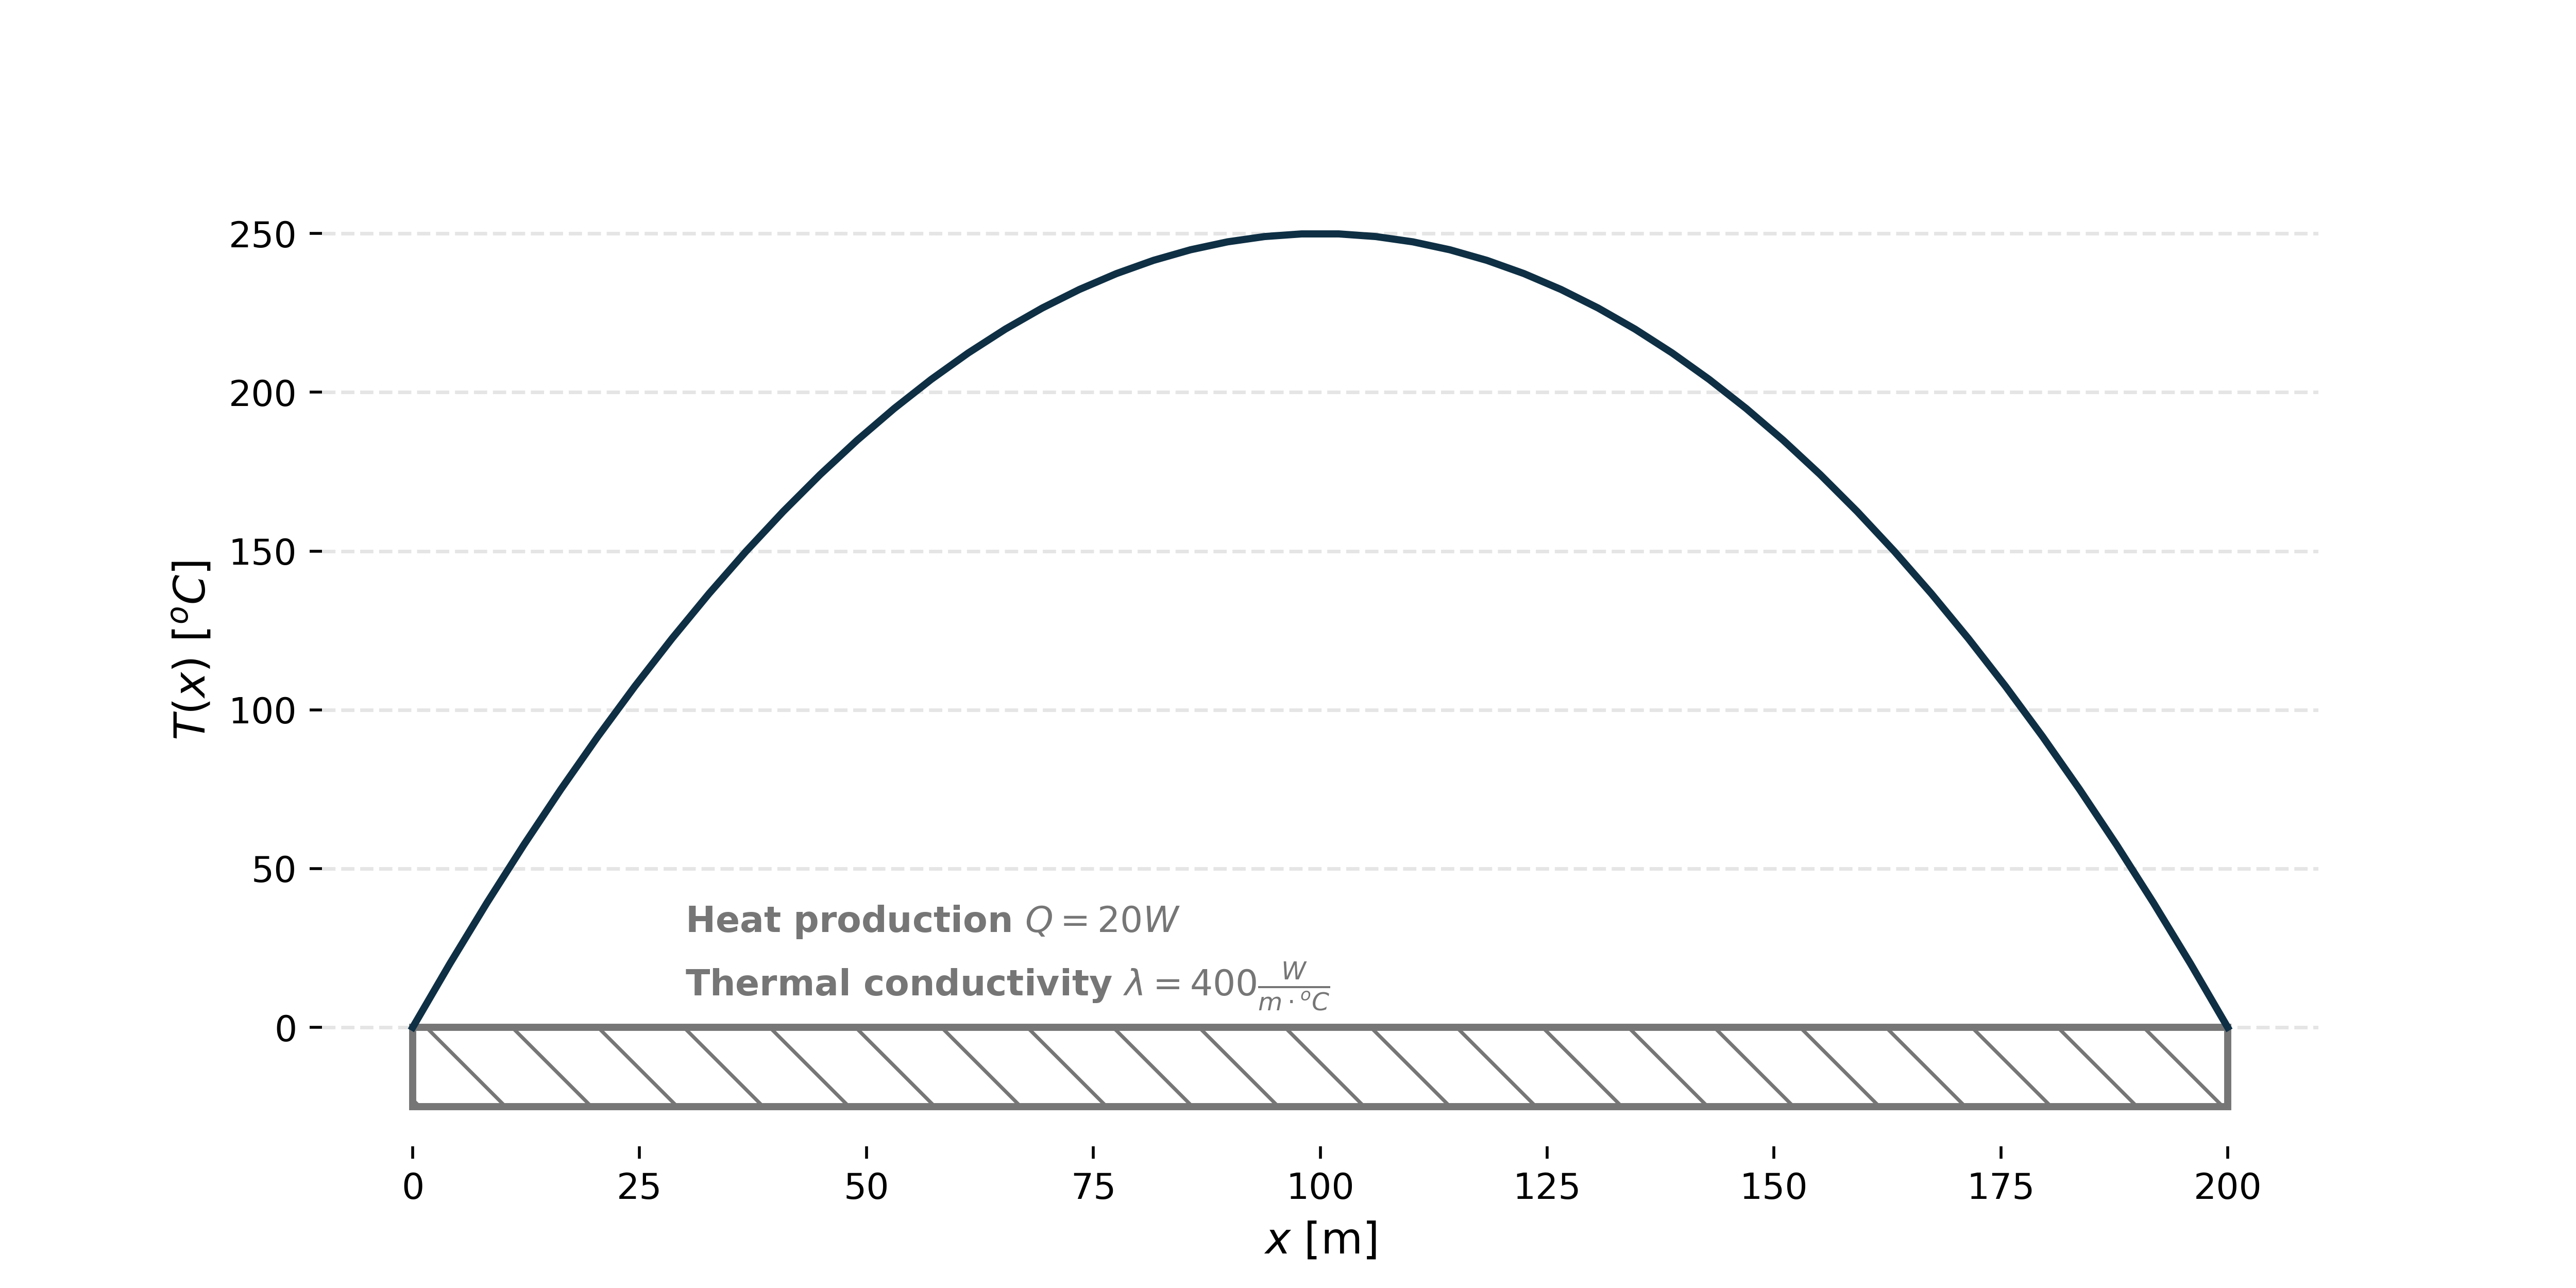
\includegraphics[width=18cm]{temperature_distribution.png}
\caption{Temperature distribution in a rod with internal heat production of $20 W$}
\label{fig:learning_curve}
\end{figure}




\setlength{\parskip}{0.0em}
\setlength{\parindent}{0cm}

\newpage

\thispagestyle{empty}

\vspace*{1cm}

This material was created by or adapted from material posted on the DelftX website, delftx.tudelft.nl, and created by TU Delft faculty members Robert Mudde, Professor of Multiphase Flow at Chemical Engineering and Peter Hamersma, Associate professor in the Dept. of Chemical Engineering, 2015. DelftX is not responsible for any changes made to the original materials posted on its website and any such changes are the sole responsibility of Kamila Zdybał.

This material is subjected to copyright by Delft University of Technology and is licensed under a Creative Commons Attribution-NonCommercial-ShareAlike 4.0 International License.

https://creativecommons.org/licenses/by-nc-sa/4.0/

\begin{center}
\vspace*{5cm}

This document was prepared as part of the course 

\textit{The Basics of Transport Phenomena} from Delft University, 

available on edX.org as DelftX: TP101x.

Copyright \textcopyright \, K. Zdybał, 2018

For more projects similar to this one

visit me on GitHub: \verb|@camillejr|

\verb|camillejr.github.io/science-docs/|

To contact me personally drop me a line at:

\verb|kamilazdybal@gmail.com|

\vspace*{2cm}

\verb|Conduction in a rod with internal heat production|

\verb|version 1.0|

Typeset with \LaTeX

\vspace*{1.8cm}

\noindent This work is licensed under the Creative Commons

Attribution-NonCommercial-ShareAlike 4.0 International 

(CC BY-NC-SA
4.0) license.
\end{center}

\end{document}